\chapter{Problem Statement} \label{chap:problem_statement} \minitoc

\section*{}

This chapter describes the problem, as can be seen in Section \ref{sec:current_issues}. In Section \ref{sec:desiderata} it is presented the wanted features for the proposed solution and in Section \ref{sec:scope} the scope of the project is defined. Section \ref{sec:main_hypothesis} contains the hypothesis this dissertation presents. The experimental methodology is outlined in Section \ref{sec:exp_meth}. Chapter \ref{sec:planning} contains a Gantt chart with the planning of this dissertation. Finally, this chapter is summarized in Section \ref{sec:stat_summary} with an overview of the topics mentioned before.

\section{Current Issues}\label{sec:current_issues}

Chapter \ref{chap:sota} contains several solutions that provide a decentralized architecture in visual programming tools applied to the Internet-of-Things paradigm. However, some of these tools solve specific problems or make assumptions regarding the scale of the system and the constraints of the devices.
We can define the problem in these issues:
\begin{enumerate}
    \item \textbf{Leveraging devices in the network}: since most tools use a centralized architecture, including Node-RED, they do not leverage the devices in the network. Fog Computing introduces a decentralized solution, one that can be applied to Node-RED by distributing the computational tasks across the edge devices.
    \item \textbf{Communication of computational capabilities}: some of the current tools require the developer to manually introduce the resources of each device in the network, which is not a scalable solution. Others have a specific list of services, manually inserted, that the devices can provide. Information about the computational capabilities of the devices in the network is vital for the successful distribution of computation across the devices.
    \item \textbf{Detecting non-availability}: when a device fails or becomes unavailable, it is important for the system to automatically realize and adapt. The majority of current solutions do not possess this feature, which is vital if a system aims to dynamically adapt to changes in the environment.
    \item \textbf{Code generation of sub-flows}: to truly leverage constrained devices, it is important to convert sub-flows or "tasks" into runnable code. Devices that support simple firmware capable of executing code can be used to execute blocks of code, despite their limited capabilities.
    \item \textbf{Provide self-adaption of the system}: devices can fail, as well as the connection between them or even the network. It is important for the system to discover and identify these changes and adapt to them at run-time, in order to keep functioning.
\end{enumerate}

\section{Desiderata}\label{sec:desiderata}

Desiderata is a Latin word that translates to "\emph{things wanted}". In the context of this document, this section contains requirements wanted in a solution that aims to solve all the issues identified in Section \ref{sec:current_issues}. The requirements are the following:

\begin{description}
    \item [D1: Communicate computational capabilities of devices connected] so that this information can be sent to an orchestrator that will decompose the total computation workload based on this data.
    \item [D2: Decomposition and partition of computation] so that the total computational requested can be distributed through all the devices in the network, using information about the computational capabilities and availability of the devices in the network.
    \item [D3: Convert computational tasks into runnable code] so that each computational task can be executed in edge and fog devices, which contain limited resources.
    \item [D4: Provide self-adaptation of the system] so that it can adapt to the non-availability of resources or even appearances of new devices.
\end{description}

\section{Scope}\label{sec:scope}

The focus of this dissertation is the development of a prototype that allows for a decentralized orchestration of an IoT system. Despite security being a critical feature, it is considered a secondary goal, allowing the dissertation to focus on its primary goals. The scope of the project is a home automation system, where its devices have firmware capable of running Lua code and accepting custom code. They also need to be able to communicate their capabilities to an orchestrator.

%\section{Use Cases}\label{sec:use_cases}

\section{Main Hypothesis}\label{sec:main_hypothesis}

This dissertation is built around the following hypothesis:

\begin{quote}
    \emph{``Given an IoT system with several heterogeneous devices connected, capable of running custom code, a decentralized architecture is more resilient, efficient and scalable than a centralized one.''}
\end{quote}

The attributes presented in the hypothesis will be measure against a system using the current development branch of Node-RED. These attributes consist of:

\begin{itemize}
    \item \textbf{Resilience} means the system's capability to adapt to failures and changes. It will be measured by injecting failures and measuring the Mean Time T Recover (MTTR).
    \item \textbf{Efficiency} how fast the system can execute the logic of the system, as well as communicate. The efficiency of a system is measured by the sum of the total latency of the system. 
    \item \textbf{Scalability} specifies how a system can grow in terms of devices supported while maintaining its features. This attribute will be tested by increasingly adding more devices and assessing the behavior of the system.
\end{itemize}

\section{Experimental Methodology}\label{sec:exp_meth}

In the interest of validating whether or not the solution implemented achieves the \emph{desiderata} and solves the current issues, we will develop test scenarios that use simulations. Each one of the test scenarios will be verified against the attributes mentioned in Section \ref{sec:main_hypothesis} to prove the proposed hypothesis.


\section{Planning}\label{sec:planning}

To manage the amount of work needed in the next few months, a \textit{Gantt Chart} was built. It is possible to consult it in Figure \ref{fig:gantt}. 
\begin{figure}[h]
    \caption{\textit{Gantt Chart} for this dissertation}
    \label{fig:gantt}
    \centering
    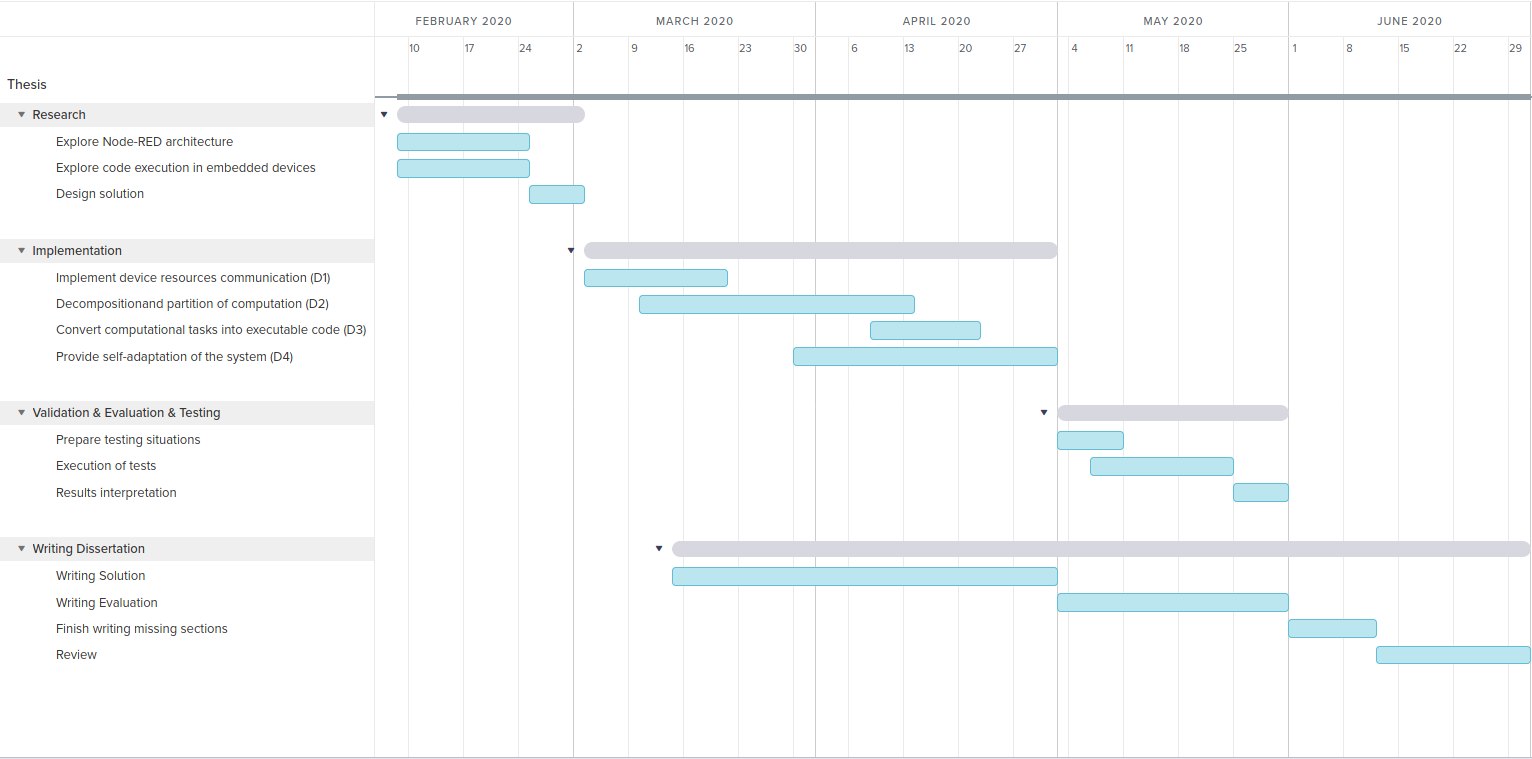
\includegraphics[width=1\textwidth]{gantt_chart_full.png}
    \end{figure}

\section{Summary}\label{sec:stat_summary}

Section \ref{sec:current_issues} starts by presenting issues and lack of features not fully present in the current tools presented in the State of the Art Chapter \ref{chap:sota}. Section \ref{sec:desiderata} presents a \textit{desiderata} that aims to fix the issues presented in Section \ref{sec:current_issues}. The hypothesis of this dissertation is presented in Section \ref{sec:main_hypothesis}, as well as an experimental methodology to prove it, in Section \ref{sec:exp_meth}. Finally, Section \ref{sec:planning} contains a Gantt Chart with the planning of the execution of this dissertation.
